
%%%%% global option for the geometry and style of the document
\documentclass[11pt,a4paper,titlepage]{article}
\usepackage[a4paper]{geometry}
\usepackage[utf8]{inputenc}
\usepackage[english]{babel}
\hyphenation{mARGOt} % to avoid the slipt of the framework name


%%%%% fancy math stuff
\usepackage{amsmath, amssymb, amsfonts, amsthm, fouriernc, mathtools}




%%%%% define new color and styles
\usepackage[dvipsnames]{xcolor}
\definecolor{MyColor1}{rgb}{0.2,0.4,0.6}
\newcommand{\textb}{\color{Black} \usefont{OT1}{lmss}{m}{n}}
\newcommand{\blue}{\color{MyColor1} \usefont{OT1}{lmss}{m}{n}}
\newcommand{\blueb}{\color{MyColor1} \usefont{OT1}{lmss}{b}{n}}
\newcommand{\red}{\color{LightCoral} \usefont{OT1}{lmss}{m}{n}}
\newcommand{\green}{\color{Turquoise} \usefont{OT1}{lmss}{m}{n}}



%%%%% handle images in the proper way
\usepackage[pdftex]{graphicx}
\graphicspath{{./pictures/}}
\DeclareGraphicsExtensions{.pdf,.jpeg,.png}
\usepackage{caption}
\usepackage{subcaption}
\captionsetup[figure]{labelfont={color=Turquoise}}



%%%%% personalize the document style
\usepackage{microtype}
\usepackage{titlesec}
\usepackage{sectsty}
\sectionfont{\color{MyColor1}}  % sets colour of sections
\subsectionfont{\color{MyColor1}}  % sets colour of sections


%%%%% set some property of the pdf
\usepackage[pdftex,hyperfootnotes=false,pdfpagelabels]{hyperref}
\pdfcompresslevel=9
\pdfadjustspacing=1
\hypersetup{%
	pdftitle={mARGOt framework user guide},%
	pdfauthor={mARGOt team}%
}


%%%%% pretty format the references
\usepackage{prettyref}
\newrefformat{fig}{Figure~\ref{#1}}
\newrefformat{tab}{Table~\ref{#1}}
\newrefformat{sec}{Section~\ref{#1}}
\newrefformat{ssec}{Section~\ref{#1}}
\newrefformat{eq}{Eq.~\ref{#1}}


%%%%% use fancy stuff for code
\usepackage{algorithmic}
\usepackage{listings}
\lstdefinelanguage{XML}
{
	basicstyle=\ttfamily\footnotesize,
	morestring=[b]",
	moredelim=[s][\bfseries\color{Maroon}]{<}{\ },
	moredelim=[s][\bfseries\color{Maroon}]{</}{>},
	moredelim=[l][\bfseries\color{Maroon}]{/>},
	moredelim=[l][\bfseries\color{Maroon}]{>},
	morecomment=[s]{<?}{?>},
	morecomment=[s]{<!--}{-->},
	commentstyle=\color{Gray},
	stringstyle=\color{RoyalBlue},
	identifierstyle=\color{ForestGreen},
	numbers=left,
	stepnumber=1,
	tabsize=2
}
\lstdefinelanguage{MyCPP}
{
	basicstyle=\ttfamily\footnotesize,
	language=C++,
	keywordstyle=\color{RawSienna}\bfseries,
	commentstyle=\color{Gray},
	stringstyle=\color{RoyalBlue},
	identifierstyle=\color{Bittersweet},
	numbers=left,
	stepnumber=1,
	tabsize=2
}


%%%%% define the actual stuff
\title{ \blue User Guide \\
	\blueb mARGOt framework}
\author{Draft version}
\date{\today}




\begin{document}

\maketitle
\thispagestyle{empty}

\tableofcontents

%\listoffigures

\clearpage
\pagestyle{plain}
\setcounter{page}{1}

\section{Introduction}


The main goal of mARGOt is to provide a dynamic autotuning framework, to enhance an application with an adaptation layer.
The mARGOt user guide, provides an high level description of the framework and example to help the integration process.
This document describes mARGOt heel, a collection of tools that aim at easing the integration process and the management of the application knowledge.
Before reading this document, we advise to go through the mARGOt user manual.


In particular, mARGOt heel is composed by two elements: the mARGOt command line interface (\textit{margot\_cli}) and the mARGOt high-level interface (\textit{margot\_if}).
margot\_cli is a tool written in python that provides utility feature to manage the application knowledge and create a simple Design Space Exploration script, based on \textit{make} files.
margot\_if is CMake-based library which generates an high-level interface of mARGOt, according to XML configuration files, using margot\_cli to generate the required glue code.
The main idea is that, provided the application requirements described in XML, it is possible to generate a simple interface, composed by few functions, to hide as much as possible implementation details of the autotuner framework.


This document is structured as follows, at first it describes the high level interface generated by margot\_if, then it describes the syntax of the related XML configuration files.
The last part of the document provides an overview of all the utility commands provided by margot\_cli.
For an example of integration, please refer to the tutorial repository on GitLab\footnote{\url{https://gitlab.com/margot_project/tutorial}}


\section{Monitors module}


The most important step in order to adapt, is to acquire insight on the current behavior of the application EFP of interest, which defines the performance of the application.
For example, the application developer might be interested on the execution time of the kernel or in the accuracy of the result.
While the first metric might be applied to every class of applications, the accuracy of the result is meaningful only in the context of an application.
For example, a video encoder might use the Peak to Signal Noise Ration (PSNR) as accuracy metric, while a scientific application might be more interested on the difference between the actual result and the ground truth value.

\begin{figure}
	\centering
	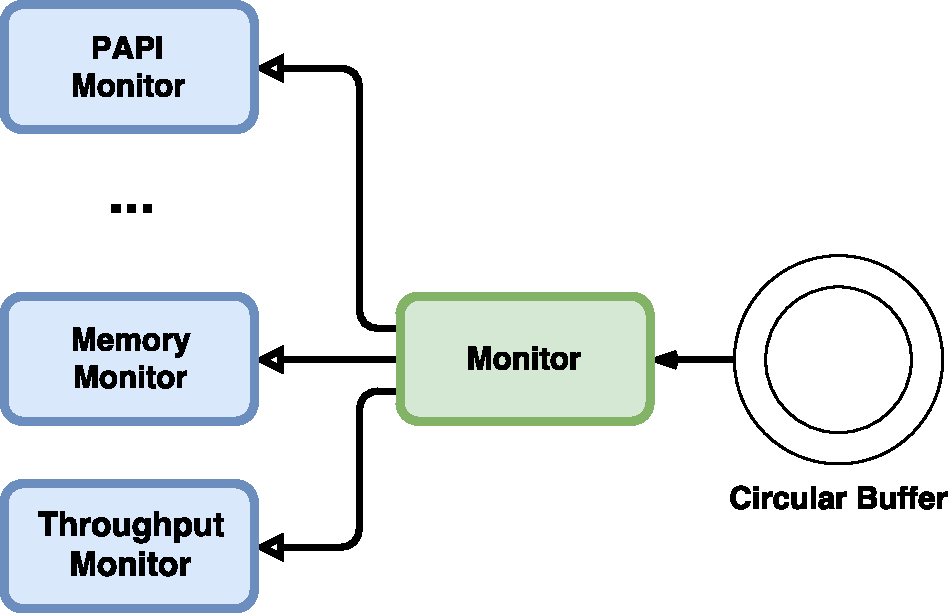
\includegraphics[scale=0.5]{monitor_modules}
	\caption{Overview of the monitors module. }
	\label{fig:monitor_module}
\end{figure}

For this reason the monitors module must be flexible enough to let the user to define custom monitor to observe application-specific metrics.
\prettyref{fig:monitor_module} shows the overview of the structure of the monitors module.
A base class (\textit{Monitor}) implements a circular buffer which store the last \textit{n} (user defined) observations and provides to the user the possibility to extract statistical properties over observed data.
Moreover, this class implements all the methods required to interact with all the other framework elements.
It is possible to specify the type of the elements stored in the circular buffer and the precision used to compute the statistical properties (by default it uses at least 32bit float).
Each time a statistical properties is computed, the monitor uses a cache-like mechanism to avoid to recompute the property.


The actual monitor must extend the latter class, with the functionality that actually gather the target metric and push the value in the circular buffer (using the \textit{push}) method.
mARGOt ships with the following suite of monitors:

\begin{itemize}
	\item Energy monitor (uses the RAPL environment)
	\item Frequency monitor (uses the CPUfreq environment)
	\item Memory monitor
	\item Odroid power monitor
	\item Odroid energy monitor
	\item PAPI monitor (uses the PAPI environment)
	\item Process and system CPU usage
	\item Temperature monitor (uses the Sensors environment)
	\item Throughput monitor
	\item Time monitor
\end{itemize}


\begin{figure}[!t]
	\centering
	\lstset{language=MyCPP}
	\begin{lstlisting}
	// monitor definitions
	margot::Monitor<float> my_float_monitor(3);
	margot::Monitor<int, double> my_int_monitor;
	margot::Monitor<double>  my_double_monitor;
	margot::TimeMonitor timer;
	
	// how to observe a metric
	timer.start();
	timer.stop()
	my_float_monitor.push(3.2f);
	
	// how to extract statistical properties
	const auto avg_time = timer.average();
	const auto avg_float = my_float_monitor.average();
	\end{lstlisting}
	\caption{Example of C++ code to define and use monitors.}
	\label{fig:monitor_examples}
\end{figure}

\prettyref{fig:monitor_examples} shows some examples on how it is possible to define and use monitors.
In particular, line 1 defines a basic monitor which stores float and has a circular buffer of three elements.
Line 2 defines a monitor of integer, however it specify that the statistical properties such as average and standard deviation should be performed using 64bit of precision. 
Moreover, the default constructor set the circular buffer size to just one element.
Line 3 defines a monitor of doubles.
Since the default type used to compute statistical properties is a float, mARGOt automatically promote the latter to double, to prevent precision loss.
Line 4 defines a time monitor, which is a specialization of the generic monitor, suitable to record the elapsed time from a start and stop method (lines 8,9).
In general each specialized monitor provides its own method to observe the target metric.
For a full description of each monitor, refer to the doxygen documentation.
To ``observe'' a value using a custom monitor (line 10), it is required to use the \textit{push} method.
Regardless of the monitor type, to extract statistical properties (lines 13-14), it is enough to use the dedicated method.
In particular, it is possible to extract the following statistical properties (defined in the enum \textit{DataFunctions}):

\begin{itemize}
	\item Average
	\item Standard deviation
	\item Maximum element observed
	\item Minimum element observed
\end{itemize}


\subsection{Application Goals}

\begin{figure}[!t]
	\centering
	\lstset{language=MyCPP}
	\begin{lstlisting}
	margot::TimeMonitor timer(margot::TimeUnit::MILLISECONDS);
	margot::Goal<int, margot::ComparisonFunctions::LESS> my_goal(2);
	
	timer.start();
	
	// application kernel
	
	timer.stop();
	
	if (my_goal.check<float,float,margot::DataFunctions::AVERAGE>(timer))
	{
		std::cout << "We are fast" << std::endl;
	}
	else
	{
		std::cout << "We should improve" << std::endl;
	}
	\end{lstlisting}
	\caption{Example of C++ code to check if the elapsed time to execute the application kernel is below $2ms$.}
	\label{fig:goal_examples}
\end{figure}

Since the application developer might have requirements on the lower bound or upper bound on a metric of interest.
mARGOt uses the class \textit{Goal} to represents this concept.
In particular, it is possible to test if a statistical properties of the monitor achieve the goal or to compute its absolute o relative error.
In the current implementation, a support four standard comparison functions (greater than, grater or equal than, less than and less or equal than), defined in the enum \textit{ComparisonFunctions}.

\prettyref{fig:goal_examples} shows an example on how it is possible to use the goals and monitors, to check if the application kernel execution time is below $2ms$.
In particular, line 1 defines a time monitor with a resolution of milliseconds.
Line 2 defines a goal with value $2$ and comparison function ``less than'', the numerical value of the goal might be changed dynamically.
After that we have instrumented the kernel of the application (lines 4-8), we check if the execution time was below $2ms$ (line 10), and we print an output message accordingly (lines 10-17). 

 
 

 
\section{Application knowledge}

The application knowledge describes the expected behavior of the application, in terms of its EFP of interest.
To represent the latter concept, mARGOt uses Operating Point objects.
An Operating Point is composed by two segments: the \textit{software knobs} segment and the \textit{metrics} segment.
The former represents a configuration of the application, the latter represents the performance reached by the application, using the related configuration.
The collection of several Operating Points define the application knowledge.
Which means that, any configuration provided by the autotuner, must be part of the application knowledge.


\subsection{Operating Point geometry}

mARGOt implements each segment of the Operating Point as an array of DataType.
The DataType is a type suitable to describe a value of either a configuration or a metric.
In particular, if the target field of the Operating Point has a known static value, we can represent such field using just its mean value.
For examples, the number of threads or the quality of the results may be fully described with a single number.
If the target field of the Operating Point is a measured metric, with a stochastic component, we must represent such field using (at least) its mean and standard deviation values.
For examples, the execution time of the kernel or its process CPU usage are a random variable, with a mean and a standard deviation.

\begin{figure}[!t]
	\centering
	\lstset{language=MyCPP}
	\begin{lstlisting}
	// define the Operating Point geometry
	using KnobsType = margot::OperatingPointSegment< 2, margot::Data<int> >;
	using MetricsType = margot::OperatingPointSegment< 2, margot::Distribution<float> >;
	using MyOperatingPoints = margot::OperatingPoint<KnobsType, MetricsType>
	
	// declare the application knowledge
	std::vector< MyOperatingPoints > application_knowledge = {
		{ // first Operating Point
			{1, 2},
			{margot::Distribution<float>(1, 0.1), margot::Distribution<float>(1, 0.1)}
		},
		{ // second Operating Point
			{2, 3},
			{margot::Distribution<float>(1, 0.1), margot::Distribution<float>(2, 0.1)}
		}
	};
	\end{lstlisting}
	\caption{Example of C++ code to define the application knowledge.}
	\label{fig:operating_point_examples}
\end{figure}

To improve the efficiency of the framework, the geometry (the C type) of the Operating Point must be known at compile-time.
In this way, mARGOt is able to exploit C++ features, to specialize the implementation of the framework according to the application knowledge.
\prettyref{fig:operating_point_examples} shows an example on how it is possible to define the application knowledge.
In particular, lines 1-4 defines the geometry of the Operating Point, while lines lines 7-16 defines the actual knowledge of the application.
In this example, the kernel has two software knobs, which values might be defined using only integer numbers (line 2).
Moreover, the application developer is interest on only two EFP, represented as a distribution of floats (line 3).
Finally, the global geometry of the Operating Point is defined in line 4.
The actual application knowledge might be represented using any STL container.
In this example, we have chosen a std::vector, brace-enclosed initialized lines(6-16).
For a full description of the Operating Point implementation, please refer to the Doxygen documentation.


\subsection{How to obtain the application knowledge}

The application knowledge is considered as an input of the framework, usually derived from a Design Space Exploration.
Since this is a well known topic in literature, the application developer is free to choose the most suitable approach to derive the application knowledge.
For example, if the design space is small, it is possible to perform a full-factorial Design of Experiment and evaluate all the possible configuration of the software knobs.
If the design space is too big, to perform an exhaustive search, it is possible to employ response surface modeling technique to derive the application knowledge.
For example, it is possible to evaluate only a subset of the design space and then interpolate the missing point.



\section{Application-Specific RunTime Manager}


\begin{figure}
	\centering
	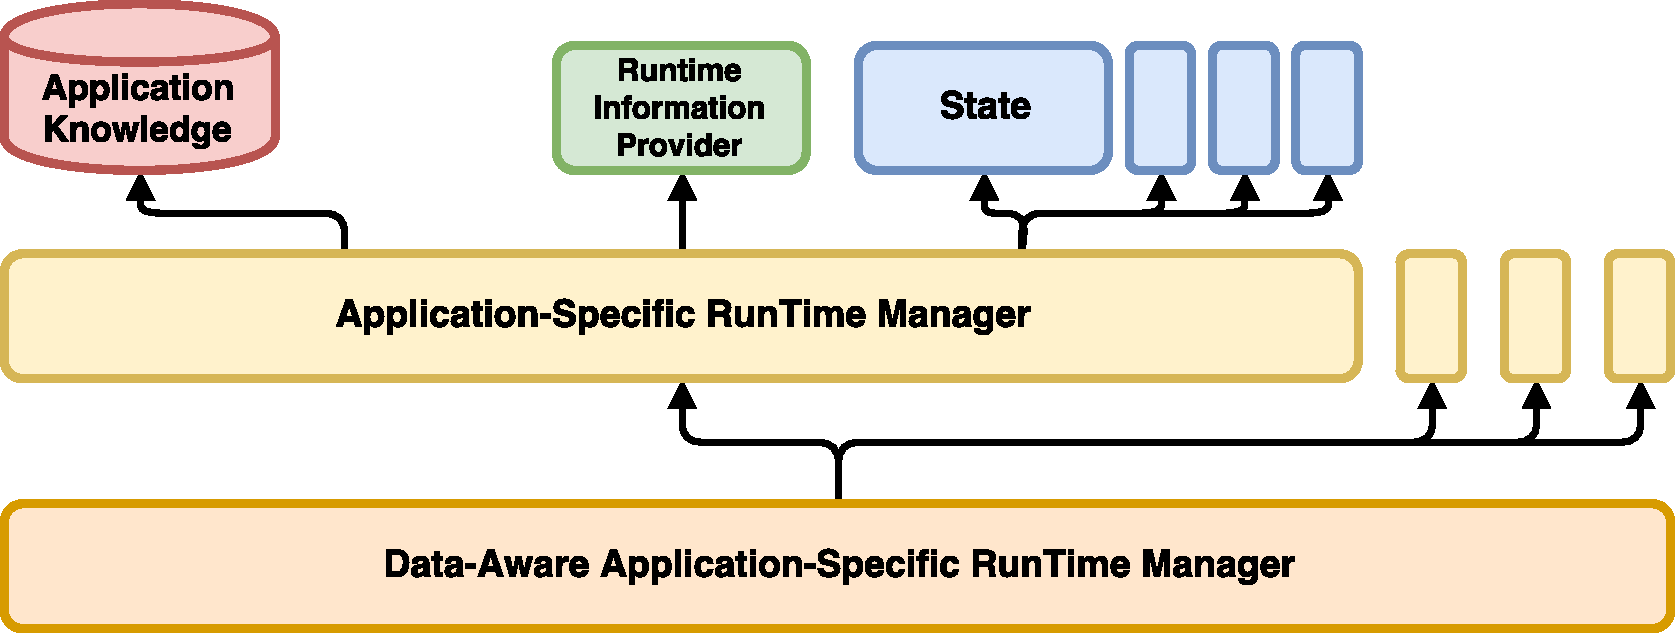
\includegraphics[scale=0.5]{asrtm}
	\caption{Overview of the manager module. }
	\label{fig:asrtm_module}
\end{figure}


This section describes the heart of mARGOt: the Manager module.
This module is in charge of selecting the most suitable configuration for the application.
\prettyref{fig:asrtm_module} shows the overall architecture of the module and the interaction between its principal elements.
In the remainder of the section, each element is explained in more details, following a bottom up approach.
However, the application developer has to interact only with the Application-Specific RunTime Manager (ASRTM) element or with the Data-Aware Application-Specific RunTime Manager element (DA-ASRTM).


\subsection{Rutime Information Provider}

This element relates the expected behavior of the application, in terms of EFPs, with the ones observed by the monitors.
In particular, since the framework will provide to the application a configuration which belong to the application knowledge, mARGOt knows the expected behavior of the application.
Therefore, if there is some difference between the expected behavior and the actual behavior of the application, the idea is that the framework must adjust the application knowledge accordingly.
To achieve this goal, the runtime information manage define the \textbf{coefficient error} $c_{e}^{i}$ for the \textit{i-th} field of the Operating Point as reported in \prettyref{eq:coefficient_error}.

\begin{equation}
\label{eq:coefficient_error}
c_{e}^{i}=\dfrac{expected_{i}}{mean_{i}}
\end{equation}

Where $mean_{i}$ represents the mean value observed by the related monitor and $expected_{i}$ represents the expected value, contained in the application knowledge.
Therefore, if $c_{e}^{i}$ is equal to $1$, it means that the $i-th$ field of the application knowledge matches perfectly with information provided by the monitor.
For numerical stability, if the observed value of the metric is exactly equal to zero, the framework adds a padding value of $1$ to the numerator and to the denominator.
In this case, $c_{e}^{i}$ tends to underestimate the actual value.

Typically, each measured value is affected by noise, produced either by the operating system or by the technique used to gather the measure.
To be robust with respect to this kind of noise, if the mean value observed by the monitor is within one standard deviation with respect to the expected mean value, we set $c_{e}^{i}$ equal to one.
The latter scenario requires that the target field is defined as a distribution in the application knowledge.
The idea is to adapt only if the difference is statistically significant.

Since some metrics may have spikes due to exceptional events, for instance when a process is migrated to another computing element, the runtime information provider store the last $n$ $c_{e}^{i}$ in a circular buffer, initially filled with ones (we assume that the application knowledge matches the reality).
The framework names \textbf{inertia} the value $n$.
If we set an high inertia to the \textit{i-th} field of an Operating Point, we are less prune to react over extraordinary events, but we are also less responsive in case of abrupt changes on the application behavior.
This parameter is exposed to the end user.


Therefore, the actual coefficient error used by the framework $\bar{c_{e}^{i}}$ is the average of all the $c_{e}^{i}$ gathered at runtime, as defined in \prettyref{eq:coefficient_error_real}.
Where $j$ indicates the \textit{j-th} $c_{e}^{i}$ in the circular buffer and $n$ indicates the inertia of the \textit{i-th} field.


\begin{equation}
\label{eq:coefficient_error_real}
\bar{c_{e}^{i}}=\dfrac{\sum_{j=0}^{n-1} c_{e,j}^{i}}{n}
\end{equation}


mARGOt uses $\bar{c_{e}^{i}}$ to perform a linear error propagation.
For examples, if with the selected configuration we expect a throughput of $10fps$, but the throughput monitor observe a throughput of $8fps$, mARGOt assumes that also all the other Operating Points will have a throughput that is $20\%$ slower than expected.
Since the error coefficient for the $i-th$ field of the Operating Point is computed in an independent way from the error coefficient of the $j-th$ field, mARGOt is able to perform a fine grained scaling of the application knowledge, to face changes in the execution environment.



\section{Integration in the target application}
\label{sec:integration}

In \prettyref{sec:asrtm} we have defined all the elements that compose the core of mARGOt.
This section aims at explaining by examples, how to integrate the autotuner in a target application.
We consider a toy application for clarity purpose.

\subsection{The target application}

\begin{figure}[!t]
	\centering
	\lstset{language=MyCPP}
	\begin{lstlisting}
	// kernel function
	void do_work( std::vector<float> input_data, const int knob );
	
	
	int main()
	{
	
		while(work_to_do())
		{
			const auto current_input = get_work();
			do_work(current_input, 2);
		}
	
	}
	\end{lstlisting}
	\caption{The C++ code of the toy application.}
	\label{fig:toy_application}
\end{figure}

\prettyref{fig:toy_application} shows the code of the toy application that we are targeting.
In particular, line 1 declares the kernel function \textit{do\_work} that we want to tune.
It takes as input the data, represented as a vector of float and a software knobs that alter the function EFPs.
In this example, we suppose that the knob performs an approximation of the computation, for instance driving the loop perforation.
Therefore, by using a small value of the knob we approximate less, while using a large number, we approximate more.
The application is defined as a main loop (lines 8-12) that continuously elaborates new inputs.
Due to the expertise of the developers, they have set a one-fit-all default value for the knob, hardcoded to the value $2$.
Obviously, we would like to manage the body of the loop.

In our example, the application developer is interested in two metrics: the execution time and quality of results.
In particular, they would like to maximize the quality of results, provided that the execution time is below a certain threshold.
Suppose that the quality of results is input independent, while the execution time depends on both, the size of the vector and the value of the software knob.


\subsection{Integration without data feature}

This section explain how to integrate mARGOt in the target application, without considering any feature of the input.
Below, it is stated the integration from the code point of view, what it lacks is the integration from the building system point view.
Since mARGOt wants to be as agnostic as possible regarding the building systems, during the compilation of the library it generates two files to help the integration of mARGOt in the building system of the target application.
In particular, it creates a \textit{FindMARGOT.cmake} file for integrating the framework in a CMake projects, while it creates a \textit{margot.pc} file for integrating the framework in projects that uses Make/autotools.



\begin{figure}[!t]
	\centering
	\lstset{language=MyCPP}
	\begin{lstlisting}
	// defining the Operating Point geometry
	using software_knob_geometry = OperatingPointSegment< 1, Data<int> >;
	using metrics_geometry = OperatingPointSegment< 2, Distribution<float> >;
	using MyOperatingPoint = OperatingPoint< software_knob_geometry, metrics_geometry >;
	
	// kernel function
	void do_work( std::vector<float> input_data, const int knob );
	
	int main()
	{
		// defining the required objects
		std::vector< MyOperatingPoint > knowledge = {
			{ // Operating Point 1
				{1},
				{margot::Distribution<float>(75.0, 1.0), margot::Distribution<float>(1.0, 0.0)}
			},
			{ // Operating Point 2
				{2},
				{margot::Distribution<float>(35.0, 2.0), margot::Distribution<float>(0.6, 0.1)}
			}
		};
		Goal<float, ComparisonFunctions::LESS> my_time_goal(50);
		TimeMonitor timer(margot::TimeUnit::MILLISECONDS, 3);
		Asrtm<MyOperatingPoint> manager;
		
		// initialize the AS-RTM
		manager.add_operating_points(knowledge);
		manager.add_runtime_knowledge<OperatingPointSegments::METRICS, 0, 5>(timer);
		manager.create_new_state("my_optimization_problem");
		manager.change_active_state("my_optimization_problem");
		using my_obj_fun = OPField<OperatingPointSegments::METRICS,
		                           BoundType::LOWER,
		                           1,
		                           0>;
		manager.set_rank< RankObjective::MAXIMIZE, FieldComposer::SIMPLE, my_obj_fun>(1.0f);
		manager.add_constraint<OperatingPointSegments::METRICS,0,3>(my_time_goal,10);
	
		while(work_to_do())
		{
			const auto current_input = get_work();
			
			// get the most suitable configuration
			manager.find_best_configuration();
			const auto best_configuration = manger.get_best_configuration();
			manager.configuration_applied();
			
			timer.start();
			do_work(current_input, best_configuration.get_mean<0>());
			timer.stop();
		}
	
	}
	\end{lstlisting}
	\caption{The C++ code of the toy application, integrated with mARGOt without using any data features}
	\label{fig:toy_application_integration_simple}
\end{figure}

\prettyref{fig:toy_application_integration_simple} shows the whole code of the application to manually integrate mARGOt in the target application.
For demonstration purpose, it exploits all the features of the AS-RTM.
For simplicity purpose we have omitted the required headers and we assume to use the namespace margot.
As you can see from \prettyref{fig:toy_application_integration_simple}, to minimize the introduced overhead, mARGOt tries to specialize as much as possible its data structures using template arguments.
 
Since in this example mARGOt doesn't use any feature of the input, it leverages the runtime information provider to react to changes in the input.
If we have few abrupt changes in the input size, mARGOt is able to sense those changes and react accordingly.

\subsubsection*{Declaring the application knowledge}
The first step to integrate mARGOt is to define the application knowledge.
In this example, we assume that the application developer performed a Design Space Exploration on the software knob, evaluating the execution time and the error using two values of the knob: $1$ and $2$.
Before defining the application knowledge, it is required to specify the Operating Point geometry (lines 1-4).
In particular, line 2 states that the each Operating Point has only one software knob, which is a integer value.
Therefore, to describe the software knob it is enough to state its mean value.
Line 3 states that each Operating Point has 2 metrics, which are a distribution of floats.
Therefore, to describe each metric it is required to state its mean value and its standard deviation.

The actual knowledge is defined later (lines 11-21) and it is composed by two Operating Points.
The first Operating Point (lines 13-16) states that when the software knob \textit{knob} is equal to $1$, the application has an execution time of $75\pm1ms$ and achieve a quality of results of $1$.
The whole list of Operating Points define the application knowledge, therefore the autotuner can select for the software knob \textit{knob} either $1$ or $2$.
In particular, after the declaration of the manger (line 24), we set the knowledge base (line 27).

\subsubsection*{Adding the runtime information provider}

Since we are not using any data feature, we exploit the feedback information of a monitor on the execution time to adapt the knowledge base, working in closed loop.
In this configuration we are able only to react to changes in the input, therefore we assume that there will be few abrut changes in the size of the input.
To achieve this behavior, we creates a time monitor with granularity of milliseconds and with a circular buffer that stores the last 3 observation (line 23); while we use an information provider with inertia $5$ on the metric with index $0$ (line 28).

\subsubsection*{Defining the optimization problem}

Given the application requirement, we need only one state which we call ``my optimization''.
Therefore, we need to create the new state (line 29), select the new state as the active one (line 30).
From now on, all the commands that alter the state refer to active one.

To define the optimization problem, we first have to define the objective function.
For simplicity, we have created an alias which refer to the average value of the second metric, thus with index $1$ (lines 31-34).
Afterward, we have defined the rank to maximize the average value of the second metric (line 35).
To represent the constraint, we need to define the related goal first (line 22), then we can add the constraint (line 36).
In particular, the latter statement creates a constraint related to the first metric, thus with index $0$.
In this example, we would like to have some confidence that the constraint is satisfied by the configuration, we created the constraint taking into account $3$ sigma of its value.
Since the goal has the relation $<$, the autotuner evaluates the upper bound of each Operating Point.
For example, the expected execution time of the second Operating Point is $41ms = 35ms + 6ms$.

\subsubsection*{Obtaining the most suitable configuration}
All the previous code was related to the initialization of the problem, to actually adapt we need to solve the optimization problem (line 43) and to retrieve the most suitable configuration (line 44).
To take advantage of the observed values, mARGOt must be notified when the application has terminated to actuate the proposed configuration.
In this example, the actuation of the configuration is trivial (line 48), therefore we can send immediately the notification (line 45).
To leverage the runtime information about the execution time, we need to profile the tuned region of code (lines 47 and 49).
The autotuner will automatically adapt according to the observed situation.



\subsection{Integration with data feature}


\begin{figure}[!t]
	\centering
	\lstset{language=MyCPP}
	\begin{lstlisting}
	// defining the Operating Point geometry
	using software_knob_geometry = OperatingPointSegment< 1, Data<int> >;
	using metrics_geometry = OperatingPointSegment< 2, Distribution<float> >;
	using MyOperatingPoint = OperatingPoint< software_knob_geometry, metrics_geometry >;
	
	// kernel function
	void do_work( std::vector<float> input_data, const int knob );
	
	int main()
	{
		// defining the required objects
		std::vector< MyOperatingPoint > knowledge_1 = // definition
		std::vector< MyOperatingPoint > knowledge_2 = // definition
		DataAwareAsrtm<MyOperatingPoint,int,
		               FeatureDistanceType::EUCLIDEAN,FeatureComparison::DONT_CARE> manager;
		
		// initialize the AS-RTM
		manager.add_feature_cluster({{100}});
		manager.select_feature_cluster({{100}});
		manager.add_operating_points(knowledge_1);
		manager.add_feature_cluster({{1000}});
		manager.select_feature_cluster({{1000}});
		manager.add_operating_points(knowledge_2);
		manager.add_runtime_knowledge<OperatingPointSegments::METRICS, 0, 5>(timer);
		manager.create_new_state("my_optimization_problem");
		manager.change_active_state("my_optimization_problem");
		using my_obj_fun = OPField<OperatingPointSegments::METRICS,
		                           BoundType::LOWER,
	 	                           1,
	                               0>;
		manager.set_rank< RankObjective::MAXIMIZE, FieldComposer::SIMPLE, my_obj_fun>(1.0f);
		manager.add_constraint<OperatingPointSegments::METRICS,0,3>(my_time_goal,10);
		
		while(work_to_do())
		{
			const auto current_input = get_work();
			
			// get the most suitable configuration
			manager.select_feature_cluster({{current_input.size()}})
			manager.find_best_configuration();
			const auto best_configuration = manger.get_best_configuration();
			manager.configuration_applied();
			
			timer.start();
			do_work(current_input, best_configuration.get_mean<0>());
			timer.stop();
		}
	}
	\end{lstlisting}
	\caption{The C++ code of the toy application, integrated with mARGOt using the data features}
	\label{fig:toy_application_integration_complex}
\end{figure}

In this scenario, we don't rely anymore on the assumption of having few abrupt changes in the input, but we allow the possibility that in each iteration of the loop we might have a different size of the input.
For this reason is not enough to be reactive, but we need to be proactive, taking into account the size of the input.
\prettyref{fig:toy_application_integration_complex} shows the integration code required.
In particular, we have defined two clusters that represent the case when we have the array of size $100$ and of size $1000$.

For the implementation point of view, the integration code is very similar.
The difference is that we need to define an Operating Point list for each cluster (lines 12-13).
The type of the manager is no more an AS-RTM, but is a DA-ASRTM (line 14,15).
In particular, beside the geometry of the Operating Points, we need to define the data feature.
In this example, we have just one data feature, which is the size of the input array, of type integer.
Moreover, we need to specify the distance type and the validity function.
In this example, we use the euclidean distance and we are just interested on choosing the closer data cluster, therefore we use the ``don't care'' enumerator.


Another difference is that, we need to create and select the data clusters (lines 18,19,21,22).
Moreover, we have to set the corresponding application knowledge (lines 20,23).
After the initialization of the autotuner, we are able to leverage the input feature, by selecting the closer data cluster for each input (line 39).
\section{Conclusion}

This document describes mARGOt, a dynamic autotuner framework, from an high-level point of view.
Moreover, it provides examples on how it is possible to enhance an application with an adaptation layer.
For a complete reference on the implementation details, please refer to the Doxygen documentation.

To further simplify the integration process, mARGOt ships with an utility tool, named \textit{margot\_cli}, which provides to the application developer additional features to ease the integration process.
In particular, it can generate an high level interface, named \textit{margot heel}, that hides as much as possible implementation details.
The guide to the utility is covered in a separate user guide.



\end{document}
